\chapter{Oefeningensessie 4}


\section{Oefening Scheduling}

Gegeven de volgende machinecode:
\begin{lstlisting}
a	ld r1, [0x8000]
b	ld r2, [0x8004]
c	add r3, r1, 1
d	mul r4, r1, r2
e	sal r5, r2, 1
f	lea r6, [0x8000 + r4]
g	div r7, r5, r3
h	add r8, r6, r3
i	mul	r9, r4, r7
j	lea r10, [0x8000 + r5]
k	add r11, r9, r8
l	add r12, r9, r10
m	ld r13, [r12]
n	st [r11], r13
\end{lstlisting}
Veronderstel ook geen geheugenafhankelijkheden, en de volgende cycli:
\begin{table}[ht]
	\centering
	\begin{tabular}{| l | l |}
		\hline 
		\textbf{Instructie} & \textbf{Cycli} \\
		\hline
		ld, st, mul & 2 \\
		div & 3 \\
		add, lea, sal & 1 \\
		\hline
	\end{tabular}
\end{table}

\begin{enumerate}
	\item Geef de data dependence graph.
	\item Schedule het basisblok op een 3-slot VLIW architectuur met 3 pipeline stages (OF, FU en WB) met operand forwarding.
	
\end{enumerate}

\section{Oefening 18.1 p431}
Gegeven de volgende flow graph

\begin{figure}[ht]
	\centering
	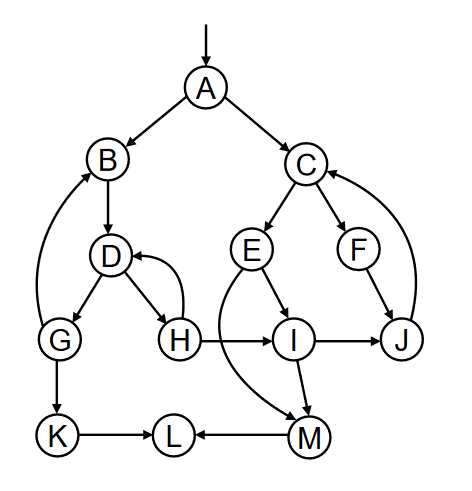
\includegraphics[width=0.5\textwidth]{ex18_1p431}
	\caption{}
	\label{fig:ex18_1p431}
\end{figure}

\begin{enumerate}
	\item Bepaal de dominators van elke node.
	\begin{table}[ht]
		\centering
		\begin{tabular}{l | l | l}
			Knoop & Iteratie 1 & Iteratie 2 \\
			A & \{A\} & \{A\} \\
			B & \{A, B\} & \{A, B\} \\
			C & \{A, C\} & \{A, C\} \\
			D & \{A, B, D\} & \{A, B, D\} \\
			E & \{A, C, E\} & \{A, C, E\} \\
			F & \{A, C, F\} & \{A, C, F\} \\
			G & \{A, B, D, G\}&\{A, B, D, G\} \\
			H & \{A, B, D, H\}&\{A, B, D, H\} \\
			I & \{A, I\}& \{A, I\}\\
			J & \{A, J\}& \{A, J\\
			K & \{A, B, D, G, K\}& \{A, B, D, G, K\}\\
			L & \{A, B, D, G, K, L\}& \{A, L\}\\
			M & \{A, M\}&\{A, M\} \\
		\end{tabular}
	\end{table}
	\item Geef de immediate dominator tree (figuur \ref{fig:ex18_1p431_idom}).
	\begin{figure}[ht]
		\centering
		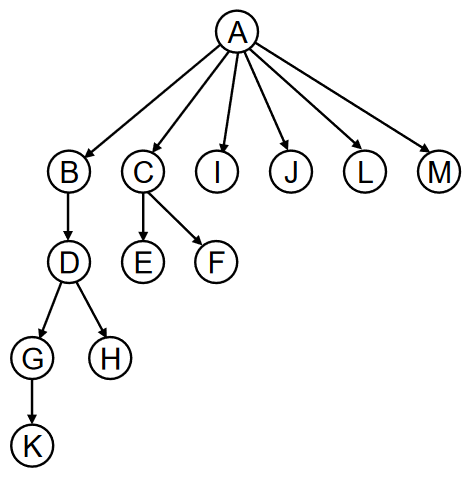
\includegraphics[width=0.7\textwidth]{ex18_1p431_idom}
		\caption{}
		\label{fig:ex18_1p431_idom}
	\end{figure}
	\item Identificeer de verzameling van nodes van elke natuurlijke lus.
	\begin{enumerate}
		\item De back edge $G \rightarrow B$ is een natuurlijke lus met als header $B$ en $S = \{B, D, G, H\}$.
		\item De back edge $H \rightarrow D$ is een natuurlijke lus met als header $D$ en $S = \{D, H\}$.
		\item De back edge $J \rightarrow C$ is geen natuurlijke lus want $C$ is geen dominator van $J$.
	\end{enumerate}
\end{enumerate}

\section{Oefening Static Single Assignment}
Gegegeven het volgende programma:

\begin{lstlisting}
1   void check_chars(int nchars, char *a, char *p) {
2 	  int i, j;
3     i = j = nchars;
4     while(j >= 1 && i <= len(a)) {
5       if (a[i] == p[j]){
6         i--;
7         j--;
8         if (j == 3) break;
9       } else {
10        if (nchars -j + 1 > floor(a[i])) {
11          i = i + nchars - j + 1;
12          continue;
13        }
14        else
15          i = i + ceil(a[i]);
16        j = nchars;
17	    }
18	  }
19  }

\end{lstlisting}

\begin{enumerate}
	\item Bouw de CFG en toon de expressies in elke knoop.
	\item Bouw de dominator tree.
	\item Bereken de dominance frontier van de while en if knopen.
	\item Maak gebruik van de dominance frontier om te bepalen waar er $\phi$ kopen toegevoegd moeten worden.
\end{enumerate}